% =============================================================================
% COPYRIGHT AND DISCLAIMER
% =============================================================================
% This file is provided as a convenience template for competition participants.
% By using it, you accept full responsibility for compliance with all applicable
% copyright, licensing, and usage rules of the Association for Computing
% Machinery (ACM) and of any LaTeX packages you load (including, without
% limitation, the "acmart" document class and related ACM materials).
%
% Consult ACM's official publication, template, and copyright policies before
% using this setup for any purpose other than this competition. Do not assume
% that this template may be reused, redistributed, or submitted elsewhere
% without independently verifying ACM's current rules.
%
% Use of the "acmart" class, the "sigconf" option, or ACM-style formatting in
% this template does NOT mean that this report, this competition, its organizers,
% or any resulting PDF is sponsored, endorsed, affiliated with, or published by
% ACM. ACM trademarks and branding remain the property of ACM.
%
% Template packages live in preamble.tex.
% Citations live in main.bib. Edit this file with your paper content.
% =============================================================================
% Team "Umer Gulzar": our references are in ours.bib (upload it next to main.bib in the Overleaf project).

\documentclass[sigconf]{acmart}
\input{preamble}
\usepackage{booktabs}
\usepackage{tikz}
\usetikzlibrary{arrows.meta,positioning}
\setlength{\emergencystretch}{1.5em}

% Guide styling: \guideStyletrue = show gray italic hints; \guideStylefalse = omit them
% \guideStyletrue
\guideStylefalse

\begin{document}

\title{Soft Multi-Annotator Targets, DINOv3 Members and PQ-Additive Instance Selection}  % Replace this with your title
\subtitle{A Solution to the Solar Filament Segmentation Challenge 2026} % DO NOT CHANGE


\author{Haseeb Khan}
\affiliation{%
  \country{Pakistan}
}
\email{EMAIL-HASEEB}   % <- Replace with your own email

\author{Muhammad Umer}
\affiliation{%
  \country{Pakistan}
}
\email{EMAIL-UMER}  % <- Replace with your own email

\begin{abstract}
    This report describes our solution to the Solar Filament Segmentation Challenge~2026, a Kaggle competition on automatic segmentation of solar filaments in GONG H-$\alpha$ observations. Two annotators of the same image agree at only PQ $=0.340$ under the competition metric, so annotator disagreement, not pixel accuracy, bounds every honest system. We train U-Nets with ImageNet and DINOv3 encoders on soft consensus targets, and we show that PQ is exactly additive over disjoint predicted instances. This turns post-processing into an exact optimisation: a pool of instance hypotheses with a learned fragment linker is ranked by a stacked LightGBM scorer that predicts each candidate's expected per-annotator IoU. The final system reaches a nested out-of-fold PQ of 0.448 (95\,\% CI 0.438--0.457) on the 707 training images and 0.39 on the public leaderboard (team ``Umer Gulzar'').
\end{abstract}

\maketitle


% ==================================== %
%              INTRODUCTION            %
% ==================================== %
\section{Introduction}
    This report goes over the details of our submitted solution to the Solar Filament Segmentation Challenge~2026 \cite{filament-segmentation-2026}. The challenge, launched on July~10,~2026, is organized by the Earth-Space AI Research (ESAIR) Lab\footnote{\href{https://www.esairlab.com/home}{www.esairlab.com/}}. This challenge utilizes the MAGFiLO dataset for evaluation of the segmentation algorithms \cite{ahmadzadeh2024dataset}. The training set has 707 full-disk $2048^2$ images with 1{,}154 annotation sets (411 images have one annotator, 145 two, 151 three) and 8{,}199 filament polygons (median area 1{,}228\,px). Predictions are scored with Panoptic Quality (PQ) \cite{kirillov2019panoptic} separately against every annotation set of an image, with TP, FP and FN pooled over all sets. Code, weights and a reproduction notebook: \url{https://github.com/umerkang66/solar-filament-segmentation}.


% ==================================== %
%              METHODOLOGY             %
% ==================================== %
\section{Methodology}\label{sec:methodology}

\begin{figure*}[t]
\centering\footnotesize
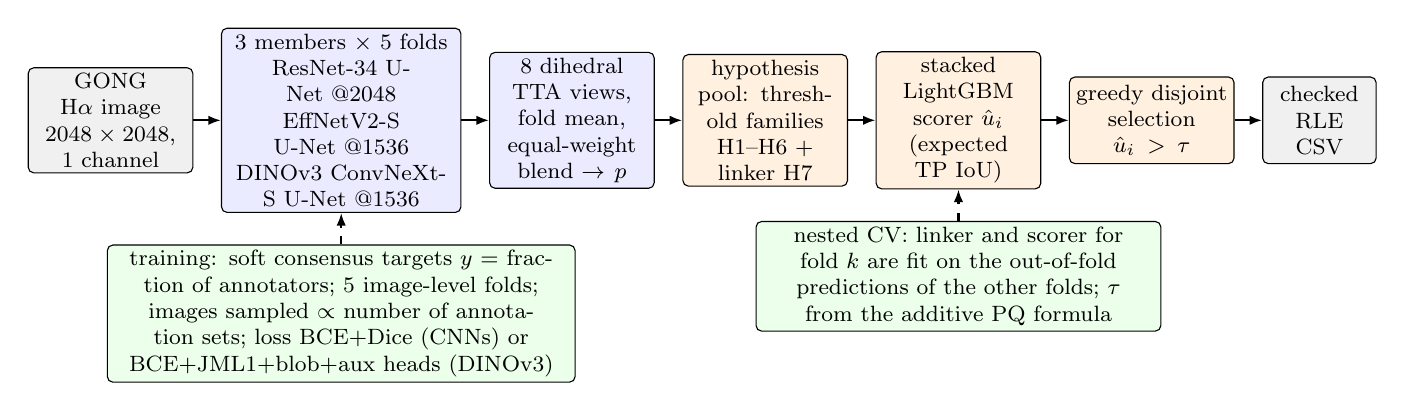
\begin{tikzpicture}[node distance=3.5mm, every node/.style={font=\footnotesize, align=center},
  box/.style={draw, rounded corners=2pt, fill=#1, minimum height=11mm, inner sep=2pt, text width=19.5mm},
  box/.default=white, arr/.style={-{Latex[length=1.6mm]}, thick}]
\node[box=gray!12] (img) {GONG H$\alpha$ image\\$2048\times2048$, 1 channel};
\node[box=blue!8, right=of img, text width=29mm] (mem) {3 members $\times$ 5 folds\\ResNet-34 U-Net @2048\\EffNetV2-S U-Net @1536\\DINOv3 ConvNeXt-S U-Net @1536};
\node[box=blue!8, right=of mem] (tta) {8 dihedral TTA views, fold mean, equal-weight blend $\rightarrow p$};
\node[box=orange!12, right=of tta] (pool) {hypothesis pool: threshold families H1--H6 + linker H7};
\node[box=orange!12, right=of pool] (sc) {stacked LightGBM scorer $\hat u_i$ (expected TP IoU)};
\node[box=orange!12, right=of sc] (sel) {greedy disjoint selection $\hat u_i>\tau$};
\node[box=gray!12, right=of sel, text width=13mm] (csv) {checked RLE CSV};
\foreach \a/\b in {img/mem, mem/tta, tta/pool, pool/sc, sc/sel, sel/csv} \draw[arr] (\a) -- (\b);
\node[box=green!8, below=4mm of mem, text width=58mm] (tr) {training: soft consensus targets $y$ = fraction of annotators;
5 image-level folds; images sampled $\propto$ number of annotation sets; loss BCE+Dice (CNNs) or BCE+JML1+blob+aux heads (DINOv3)};
\node[box=green!8, below=4mm of sc, text width=50mm] (ne) {nested CV: linker and scorer for fold $k$ are fit on the out-of-fold predictions of the other folds; $\tau$ from the additive PQ formula};
\draw[arr, dashed] (tr) -- (mem);
\draw[arr, dashed] (ne) -- (sc);
\end{tikzpicture}
\caption{End-to-end pipeline. Top: inference (blue: networks, orange: instance stage). Bottom: how the learned parts are trained.}
\label{fig:pipeline}
\end{figure*}

\textbf{Metric analysis.} If predicted masks are disjoint, a GT filament can be hit (IoU $>0.5$) by at most one prediction. Hence for any subset $S$ of predicted instances
\begin{equation}
\mathrm{PQ}(S)=\frac{\sum_{i\in S} a_i}{\tfrac12 N_{gt}+\sum_{i\in S} d_i},
\end{equation}
where $a_i$ is the sum of instance $i$'s TP IoUs over the $m_i$ annotation sets of its image and $d_i=m_i/2$. Adding $i$ raises PQ if and only if its expected per-annotator TP IoU $u_i=a_i/m_i$ exceeds PQ$/2\approx0.22$. Once instances are extracted, every threshold and filter search is an exact sum, and $u_i$ is a regression target for instance scoring. The metric also counts overlapping duplicates as extra TPs (each mask twice would raise our out-of-fold PQ from 0.439 to 0.483); we submit strictly disjoint masks.

\textbf{Pre-processing and targets.} Images are decoded once and normalised (mean 125, std 18). Every polygon is rasterised with pycocotools, exactly like the ground truth. The training target of a pixel is the fraction of the image's annotators covering it (soft consensus). For the DINOv3 member we add a soft skeleton, a soft core and one instance map per annotation set. Only the \texttt{segmentation} field is used.

\textbf{Networks.} All members see the full solar disk. Two are U-Nets \cite{ronneberger2015unet} with scSE decoder attention \cite{roy2018scse} on ImageNet encoders: ResNet-34 \cite{he2016resnet} at 2048\,px and EfficientNetV2-S \cite{tan2021efficientnetv2} at 1536\,px, trained with BCE + soft Dice. The third (M5) is a U-Net on a DINOv3 \cite{dinov3} ConvNeXt-S \cite{liu2022convnext} encoder at 1536\,px, with a GroupNorm/GELU/scSE decoder, a light stride-1/2 detail stem, skeleton and core heads and deep supervision. It is trained with BCE + the Jaccard metric loss JML1 \cite{wang2023jml}, which is minimised at $P=y$ for soft labels, plus a blob loss \cite{kofler2023blob} over the instances of one sampled annotation set, so that every filament counts equally as in PQ. A 5-fold proxy ablation with a paired bootstrap gate chose this loss: BCE+Dice 0.386, BCE+JML1 0.386, full loss 0.396 ($+0.009$, 90\,\% CI $[+0.006,+0.012]$).

\textbf{Sampling and splits.} We use 5 image-level folds (seed 42): all annotation sets of an image share a fold, and each image is out-of-fold exactly once. Images are drawn in proportion to their number of annotation sets, as the metric weights them. Augmentation runs on the GPU (arbitrary rotation, flips, scale 0.87--1.15, shift, gamma, contrast, blur, noise). Training: AdamW, warm-up and cosine decay, batch 8, bf16, weight EMA 0.998, 60--80 epochs; the DINOv3 encoder uses a 5$\times$ lower learning rate. The test set is never used for training or tuning.

\textbf{Post-processing (Stage C).} Maps are averaged over 8 dihedral views and the 5 fold models of each member, then over the members. Hypothesis families H1--H6 cut the map at several seed and extent thresholds; seeds within ${\sim}16$\,px are grouped into one filament, because annotators draw one polygon around a broken filament ($+0.008$ PQ). A learned fragment linker (LightGBM on pairs of components) adds H7 at two link thresholds. A stacked LightGBM scorer predicts $u_i$ from probability, contrast, shape, position and context features of every candidate. A greedy selection keeps candidates with $\hat u_i>\tau$ in descending order, allowing at most 5\,\% overlap with already kept masks and removing it. The linker and the scorer are trained with nested cross-validation (Fig.~\ref{fig:pipeline}).

\begin{figure*}[t]
\centering
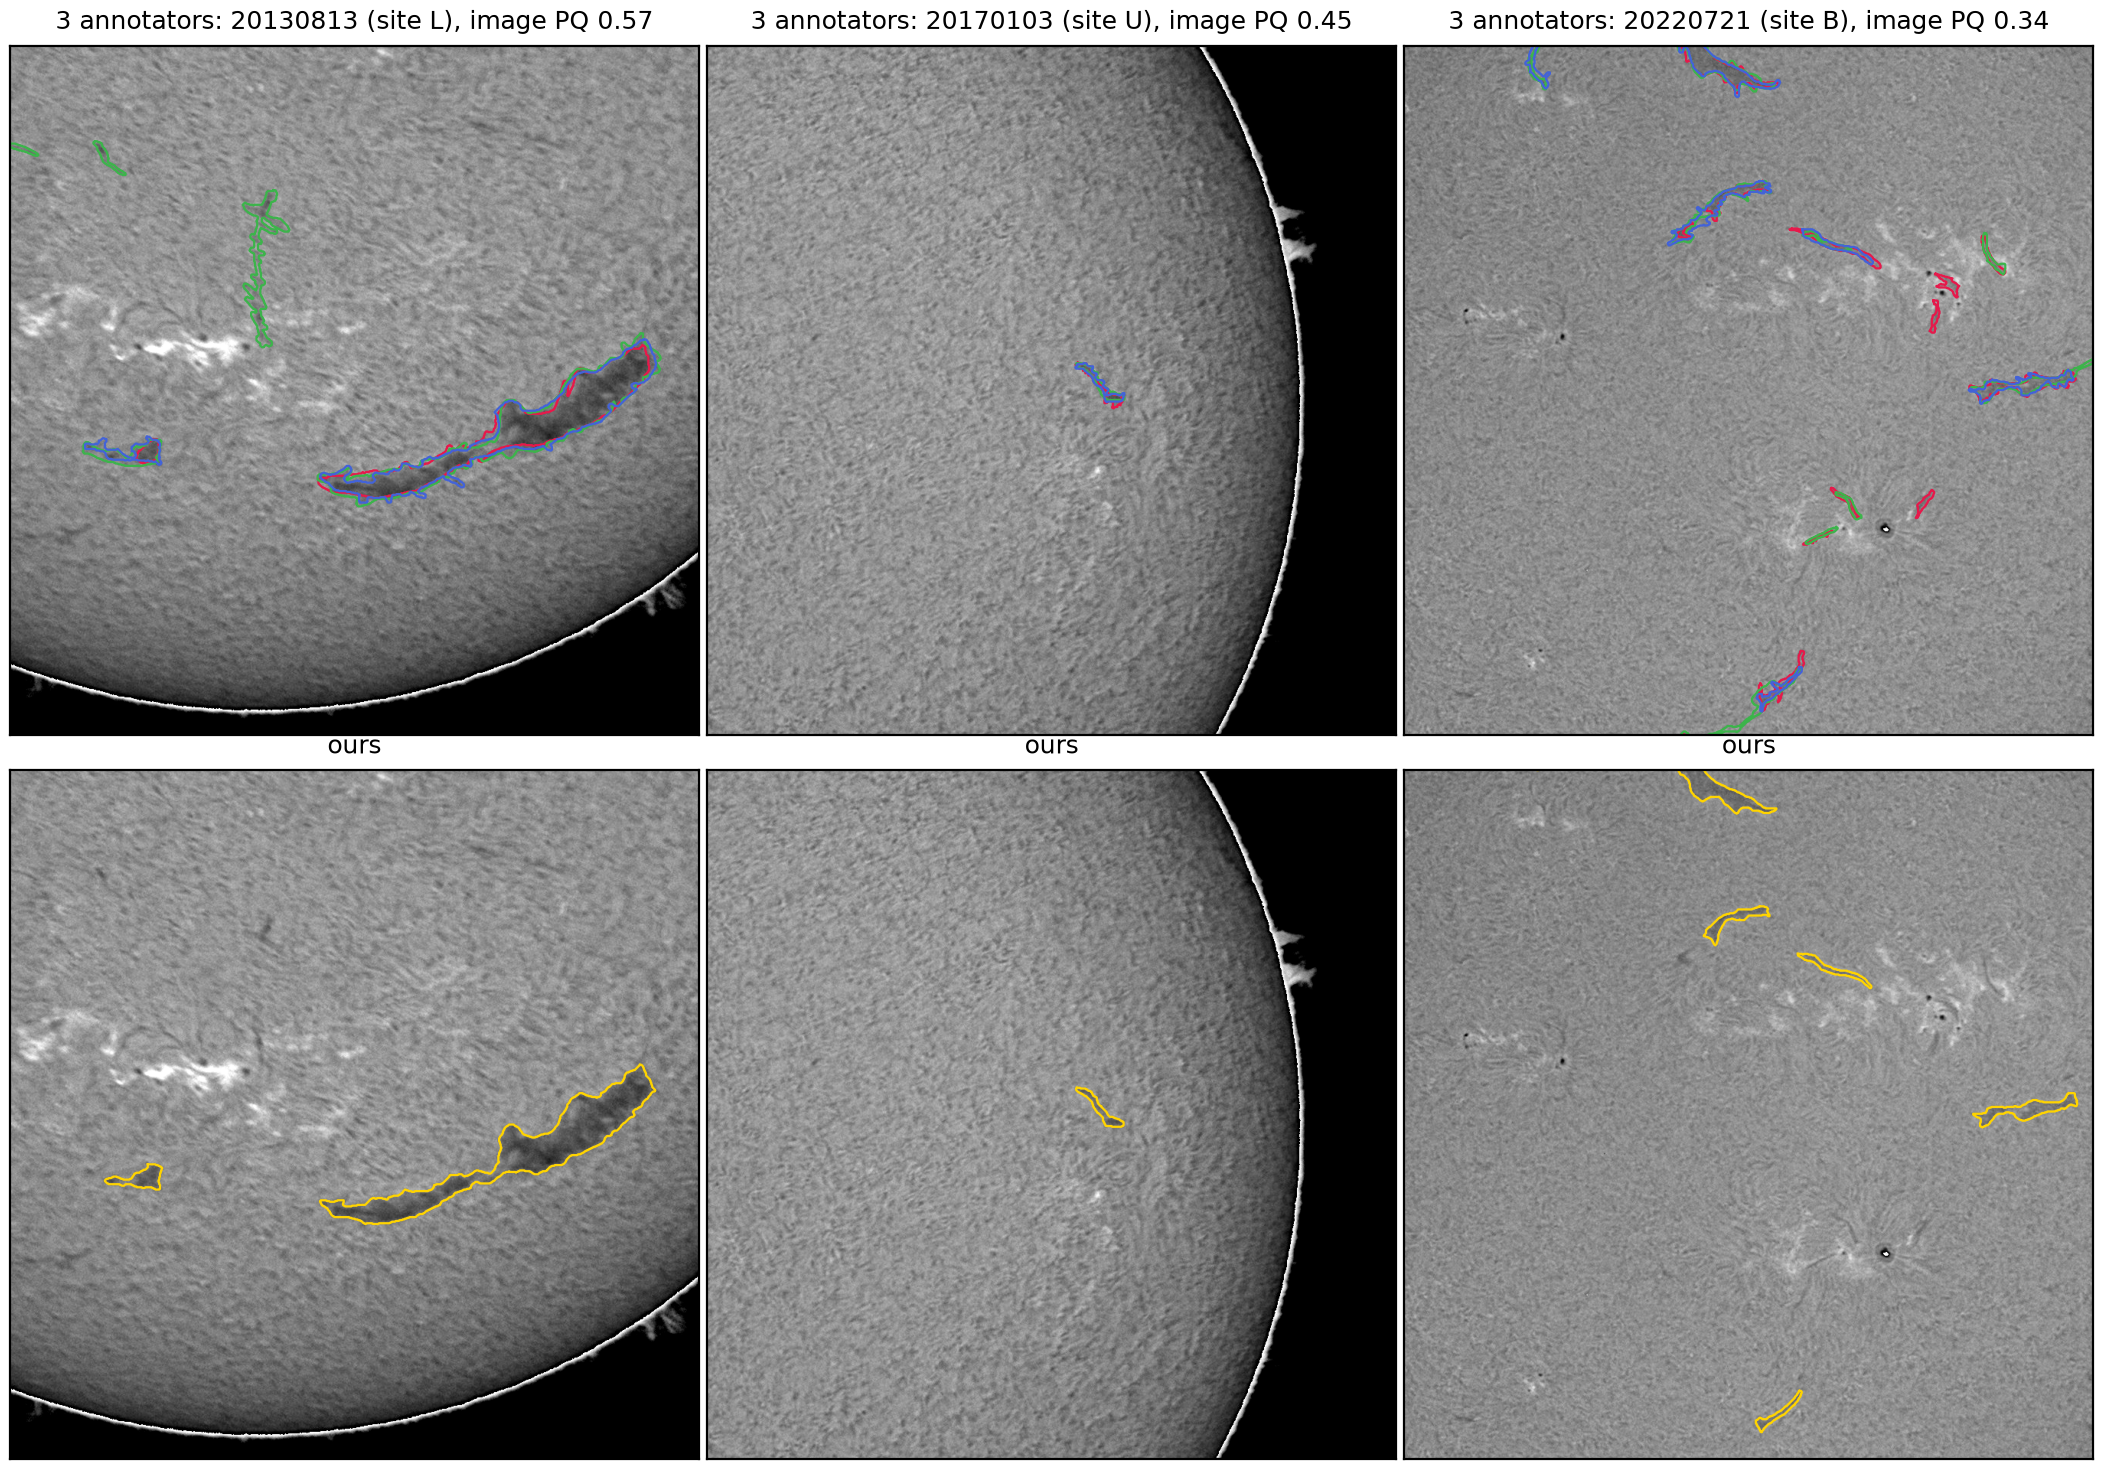
\includegraphics[width=0.86\textwidth]{figures/examples.png}
\caption{Out-of-fold examples on 3-annotator training images at the 85th, 50th and 15th percentile of per-image PQ (left to right; crops of $900\times900$\,px). Top: the three annotators' polygons, one colour each. Bottom: our prediction.}
\label{fig:examples}
\end{figure*}

\begin{figure*}[t]
\centering
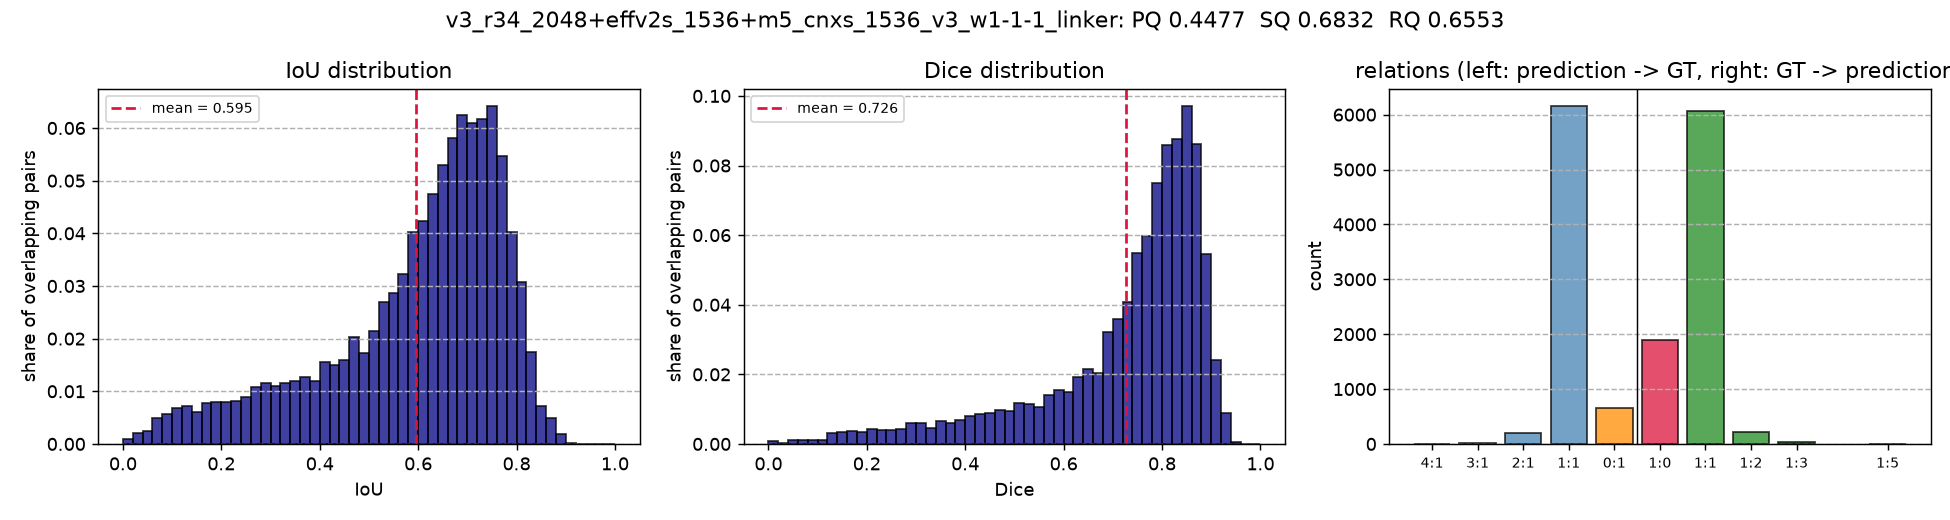
\includegraphics[width=\textwidth]{figures/rubric_final.png}
\caption{Final system, out-of-fold: IoU and Dice of overlapping prediction--GT pairs, and the relations between predictions and GT filaments (left: predictions per GT count, right: GT per prediction; 1:1 dominates, 1:$n$ and $n$:1 are rare).}
\label{fig:rubric}
\end{figure*}

% ==================================== %
%              EVALUATION              %
% ==================================== %
\section{Evaluation}\label{sec:evaluation}
\textbf{Strategy.} All numbers are out-of-fold on the 707 training images with the organisers' metric (our implementation matches their notebook pair by pair). Learned stages are nested, so only the two global thresholds of the selection are tuned on the reported predictions. Uncertainty: 95\,\% percentile intervals from 2{,}000 bootstrap resamples of images, and the spread of PQ over the 5 folds.

\begin{table}[t]
\caption{Human agreement, ceilings and our system.}\label{tab:ceil}
\centering\footnotesize
\begin{tabular}{@{}lccc@{}}
\toprule
reference & PQ & SQ & RQ \\
\midrule
annotator vs.\ annotator (same image) & 0.340 & 0.634 & 0.536 \\
consensus of 2 vs.\ held-out 3rd (151 img.) & 0.333 & 0.632 & 0.528 \\
oracle with all labels known (296 img.) & 0.666 & 0.825 & 0.807 \\
ours, out-of-fold (707 img.) & 0.448 & 0.683 & 0.655 \\
\bottomrule
\end{tabular}
\end{table}

\textbf{Ceilings} (Table~\ref{tab:ceil}). Even an oracle that knows every label cannot exceed 0.666 with one set of masks on multi-annotator images, because the annotators contradict each other. Our system is above human consensus because it predicts the average annotator.

\begin{table}[t]
\caption{Out-of-fold PQ with 95\,\% bootstrap CI and fold mean $\pm$ s.d.; public leaderboard (LB).}\label{tab:results}
\centering\footnotesize
\setlength{\tabcolsep}{3pt}
\begin{tabular}{@{}lccc@{}}
\toprule
system & PQ [95\,\% CI] & folds & LB \\
\midrule
ResNet-34 @1024, no TTA (fold 0) & 0.380 & & \\
3 U-Nets @1024/1536 + rescorer & 0.438 [0.429, 0.447] & $0.438\pm0.011$ & 0.38 \\
2 U-Nets @2048/1536 + extent sel. & 0.444 [0.435, 0.452] & $0.443\pm0.011$ & 0.38 \\
\textbf{final: + DINOv3 member, Stage C} & \textbf{0.448 [0.438, 0.457]} & $0.447\pm0.012$ & \textbf{0.39} \\
\bottomrule
\end{tabular}
\end{table}

\textbf{Results} (Table~\ref{tab:results}). The paired bootstrap of final minus the second system is $+0.0039$ [$+0.0004$, $+0.0075$]. Members alone score 0.433 (ResNet-34 @2048), 0.436 (EfficientNetV2-S) and 0.430 (DINOv3 ConvNeXt-S); per-fold validation PQ of single DINOv3 models (no TTA) is 0.37--0.41, the best single networks. Stage C adds $+0.002$ over a per-filament extent selector on the same maps; its oracle shows ${\sim}8$ points of headroom, but which extent a given annotator draws is largely unpredictable from the image. Of the overlapping prediction--GT pairs, 75.7\,\% have IoU $>0.5$ (mean IoU 0.595, mean Dice 0.726). Fragmentation (GT overlapped by 2+ predictions) is 3.0\,\% and over-merging 2.9\,\% (Fig.~\ref{fig:rubric}). Fig.~\ref{fig:examples} shows typical outputs. The final CSV is rebuilt from the released weights by the repository's notebook: running it on the server reproduced 1{,}061 of the 1{,}067 submitted masks bit-identically; 1{,}066 match with IoU $\ge0.999$ and one differs by 74\,px (IoU 0.95), as expected from non-deterministic bf16 GPU inference.

\textbf{Where PQ is lost.} 56\,\% of the lost PQ is the IoU deficit of true positives (boundary disagreement), 15\,\% missed filaments, 14\,\% wrong extent (IoU $\le0.5$), 6\,\% spurious predictions and 10\,\% fragments and merges. Small filaments ($<500$\,px: PQ 0.29, recall 0.36) and the limb ($r/R>0.8$: PQ 0.37) are the weakest groups. PQ is uniform across the six sites (0.43--0.45) and the number of annotators per image, but varies from 0.40 to 0.55 across annotator groups.

\textbf{Leaderboard gap.} Public scores are ${\sim}0.06$ below out-of-fold, as other teams also report. It is not chance (random 90-image subsets have s.d.\ 0.012 and fall to $\le0.385$ with probability $<0.0003$), not mask width (masks eroded/dilated by 1\,px score 0.37/0.35) and not calibration (test and out-of-fold maps differ by ${\sim}1$\,\% in foreground fraction). The most likely cause is an annotator shift between training and test labels. We tuned nothing on the leaderboard and never used the public MAGFiLO release, which contains labelled test images.

\textbf{Strengths and weaknesses.} Strengths: an exact, metric-aware selection with a principled keep threshold; honest nested evaluation; disjoint masks with few fragments or merges; 7\,s of post-processing for 180 images on 12 CPU workers and 0.46--0.72\,s of network inference per image and fold model on one AMD MI300X. Weaknesses: faint, small and near-limb filaments, and per-annotator extent, which no image feature predicts well. Improvements: annotator-conditioned training that models each annotator's style, semi-supervised training on unlabelled GONG frames, larger DINOv3 encoders at native resolution, and tuning extraction thresholds per blend (soft-target members are calibrated lower: our ViT-B member scores 0.441 at threshold 0.4 vs.\ 0.427 at 0.6, and a fixed 0.6 dropped it from the blend).

% ==================================== %
%            ACKNOWLEDGMENT            %
% ==================================== %
\section{Acknowledgment}\label{sec:acknowledgment}
    % Do not change
    The organization of the Filament Segmentation Challenge 2026 is partially supported by the U.S. National Science Foundation (NSF) under Grant No. 2209912 and 2433781, directorate for Computer and Information Science and Engineering (CSE), and Office of Advanced Cyberinfrastructure (OAC), and Grant No. 2511630, AST Division Of Astronomical Sciences and MPS Directorate for Mathematical and Physical Sciences.

    The Filament Segmentation Challenge 2026 is sponsored by the U.S. National Science Foundation (NSF) National Solar Observatory (NSO).

    This work utilizes GONG data obtained by the NSO Integrated Synoptic Program, managed by the National Solar Observatory, which is operated by the Association of Universities for Research in Astronomy (AURA), Inc. under a cooperative agreement with the National Science Foundation and with contribution from the National Oceanic and Atmospheric Administration. The GONG network of instruments is hosted by the Big Bear Solar Observatory, High Altitude Observatory, Learmonth Solar Observatory, Udaipur Solar Observatory, Instituto de Astrofísica de Canarias, and Cerro Tololo Interamerican Observatory.

\bibliographystyle{ACM-Reference-Format}
\bibliography{main,ours}

\end{document}
